\chapter{Data}

\section{Datasets}

\subsection{Lyrics dataset}
 \todo{Byly dalsi moznosti? Da se rict ze Lyrics datasety je tezke sehnat a tim padem jsme se spokojili s timhle mensim?}We chose the \textit{55000+ Song Lyrics dataset} from
 Kaggle.com\footnote{https://www.kaggle.com/mousehead/songlyrics} to obtain lyrics
 data. The Kaggle dataset originally contained 57 650 English songs. It’s lyrics are
 scraped from LyricsFreak\todo{link do footnote}. Extremely long and short lyrics were removed as well as
 all non-ASCII symbols from the lyrics. Figure \ref{fig:lyrics_dataset} shows the
 first two entries of the dataset.\\
 \begin{figure}[h]
    \centering
	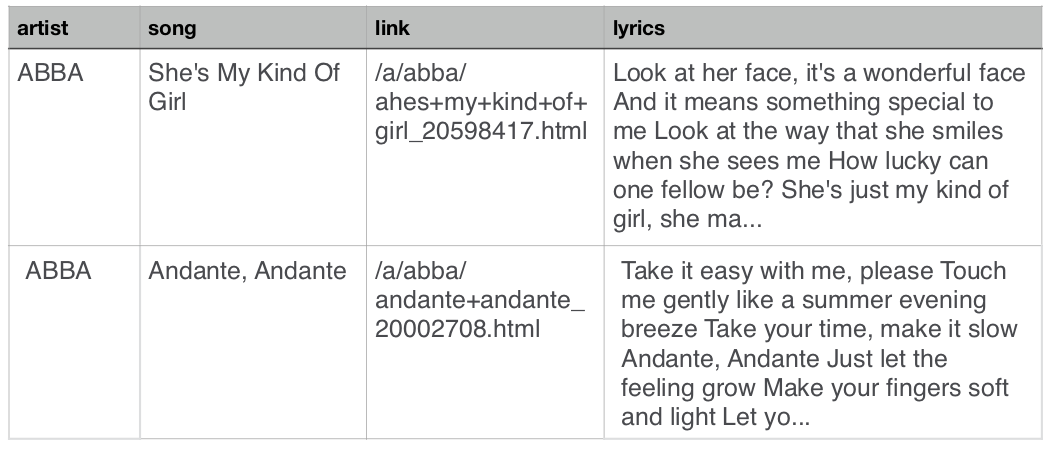
\includegraphics[height=60mm]{./img/dataset_preview.png}
	\caption{First two entries of the 55000+ Lyrics Dataset}
	\label{fig:lyrics_dataset}
\end{figure}

\subsection{User-information dataset}
To evaluate text and audio based methods on real-life user data, we had to select a
dataset containing song information and lyrics as well as a dataset with information
about users and their played tracks. First we tried to match the lyrics dataset onto
the \textit{Thisismyjam} dataset \footnote{http://www.thisismyjam.com}. However we
were able to match only 6800 songs with lyrics as well as user data. We then tried
the \textit{Echo Nest Subset profile} \cite{Bertin-Mahieux2011}
\footnote{https://labrosa.ee.columbia.edu/millionsong/tasteprofile} dataset available
on the Milion Song Dataset website. 
The Echo Nest Taste Profile Subset provides us with 48,373,586 triplets of
\textit{user id, song id} and \textit{the number of times the user has played a
song}. This then had to be mapped onto the MSD\todo{zkratka nebyla zavedena - napis ji u prvniho vyskytu} dataset to get the name and artist and
then onto our lyrics dataset.\\
After removing songs we did not have lyrics for, we ended up with 16594 unique songs,
and 45054 unique users. \todo{info o tom, ze i kdyz je to drasticka redukce, stale jeste mame dostatek dat pro provedeni experimentu} For each of the 16594 songs we also acquired a mono .wav
file. \\

\section{Final dataset statistics}
Overall our final dataset had 160454 entries containing a user id, the artist, the
song title and the lyrics. {\bf We used this to create a number of different datasets}
suited for different tasks throughout the thesis. \\
\begin{itemize}
    \item The \textit{Song dataset} denoted as SD in this work. It contained the
    16594 unique songs with their metadata, the users were omitted.
    \item The \textit{User dataset} denoted as UD. It contained 11123 unique user \todo{unique users, who have at least 4 songs in their playlists}
    id's. For each, there were at least 4 songs. This means, it is a dataset containing playlists that have at least 4 entries. 
\end{itemize}
 {\bf --As--} our  evaluation method is aimed to reveal the missing entries based on the
 implemented recommendation techniques{\bf .} \todo{Odkaz do dalsi kapitoly tu docela rusi, dal bych ho do footnote} which will be described in more detail in
 Chapter \ref{chap:experiments} {\bf (Therefore,)}we studied the dataset and especially the playlist's
 lengths in more detail.\\
Here are some important remarks:
\begin{itemize}
    \item Each user only has one playlist. This means there is a one to one mapping between users and playlists and the terms are used interchangeably.
    \item We do not know which songs the user has played most recently.
    \item Users with only one song are useless for \todo{the purpose of evaluation} our evaluation.
    \item \todo{Tohle neni az tak jasne apriori, zminil bych to spis nekde u hypotez se kterymi jsme sli do experimentu} It should be easier to complete the missing songs for users with longer playlists.
\end{itemize} 
When analyzing our dataset, it turned out, that out of 45054 playlists, there are 22257 with only one song, which leaves us with 22797 we can use. Meaning,\todo{sentence fragment} that a little over half of the playlists is useful for our evaluation.

The distribution of the lengths for useful playlists is shown in more detail in Figure
\ref{fig:playlist_length_distribution}. We can see that most of the playlists are
short, almost a third of them only contains two songs. The average number of songs
per playlists (including those containing only one song) is 3.56. 
\begin{figure}[ht]
    \centering
	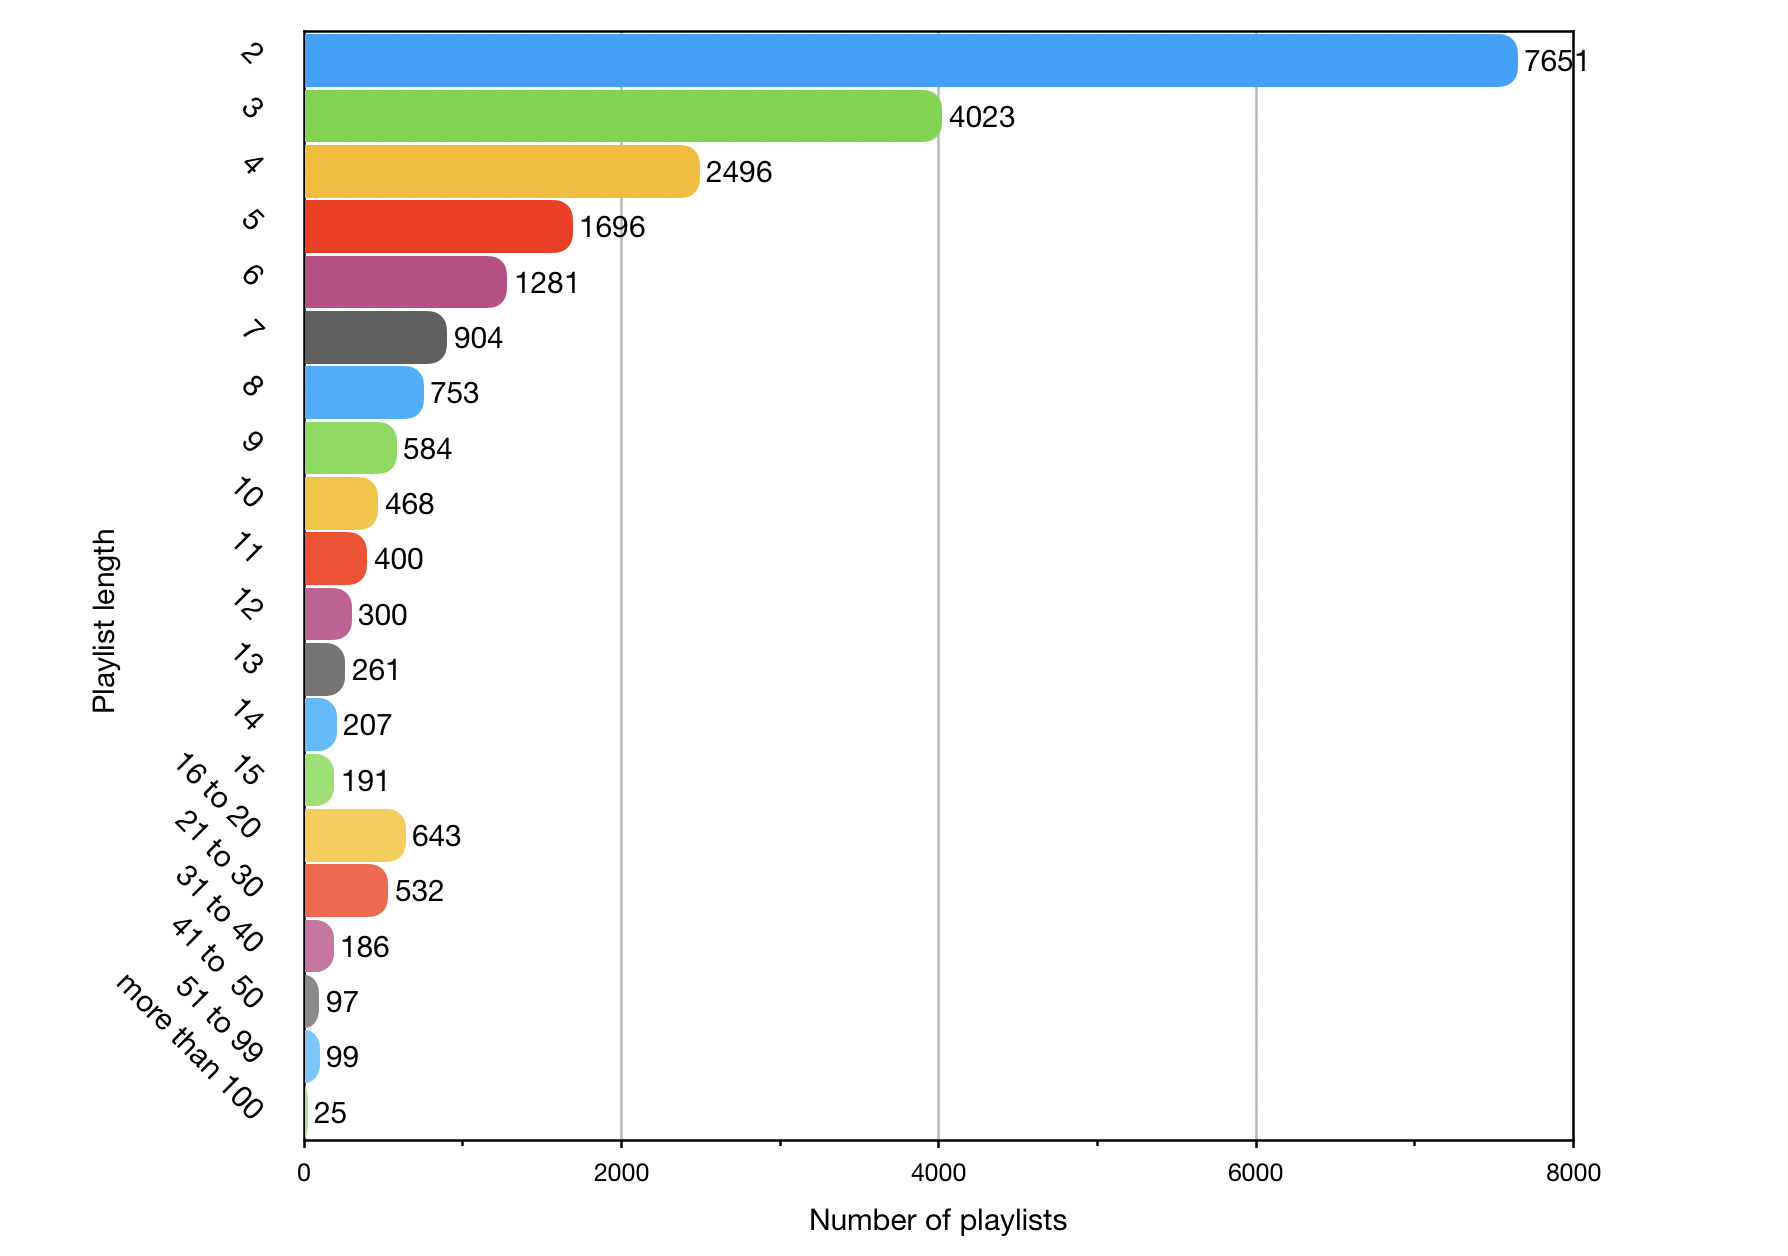
\includegraphics[width=1\linewidth]{./img/playlist_length_numbers.png}
	\caption{Playlists' lengths histogram}
	\label{fig:playlist_length_distribution}
\end{figure}

The average number of playlists a song from our dataset belongs to is 10.84. The
distribution and the most popular songs are depicted in Figure
\ref{fig:popular_song_distribution}. The by far most popular song with a total of 816
plays was \textit{Royals} by \textit{Lorde}. Second came \textit{Radioactive} by
\textit{Imagine Dragons} with 674 users who played it. All other songs have been
played by less than 500 users.

\begin{figure}[ht]
    \centering
	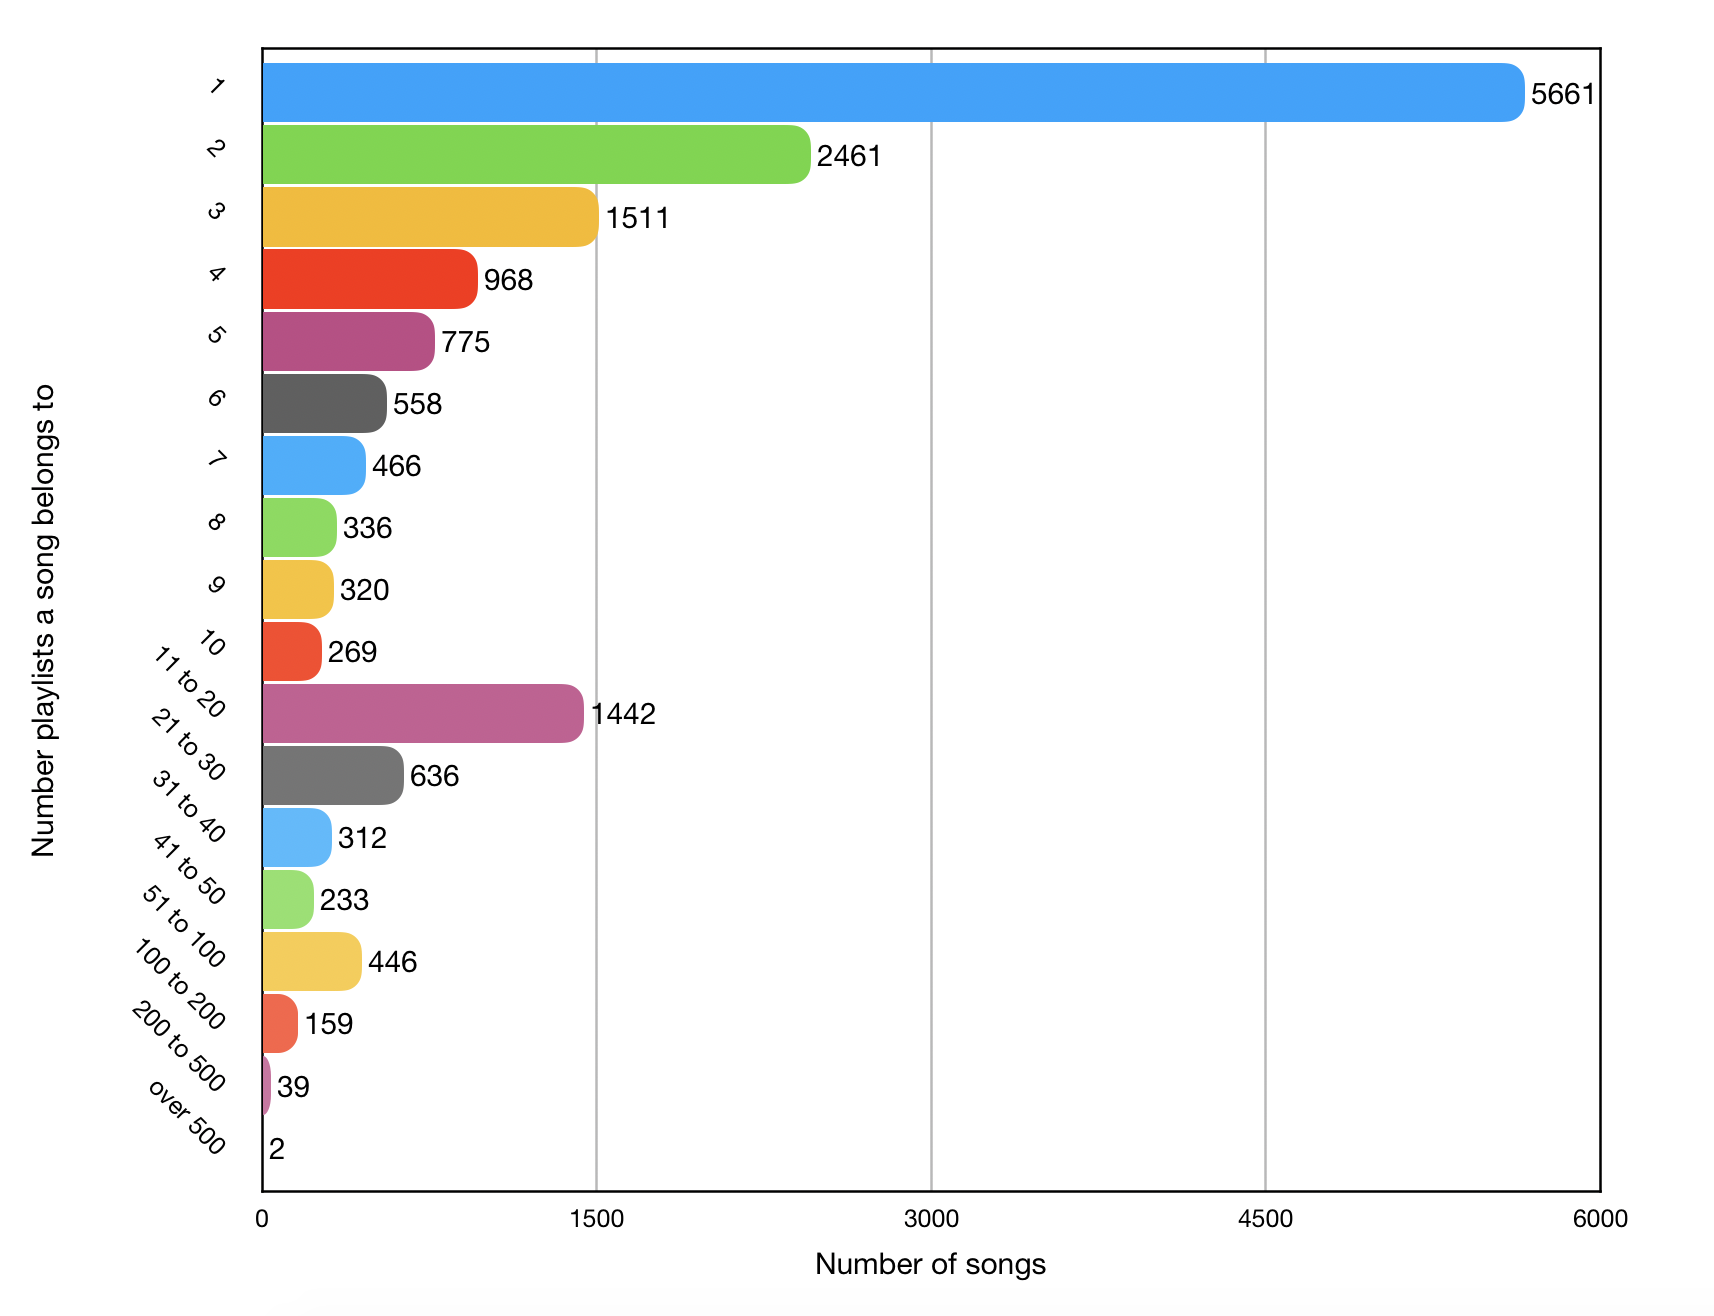
\includegraphics[width=0.8\linewidth]{./img/times_played_numbers2.png}
	\caption{The histogram of playlist counts per individual songs}
	\label{fig:popular_song_distribution}
\end{figure}
